% 关于小时百科(白皮书)
% license CCBYSA3
% type Tutor

\subsection{我们想做什么}
\subsubsection{小时百科不是另一个维基百科——百科与教学}
看到 “\textbf{小时百科}” 这个标题, 可能许多人会以为这是一个类似维基百科的网站。 但我们并不是在做一个国产的数理领域的维基百科, 虽然由于历史原因我们的项目叫做小时百科, 但目前我们主要做的是\textbf{教学}。 目前大部分内容都更接近\textbf{教材}而不是\textbf{百科}。 这和维基百科有什么区别呢?

维基百科上每个条目基本可以看做是围绕其标题的一个\textbf{综述}, 追求全面、客观、中立、一般性。 它的很多内容对初学者并不友好。 例如在维基百科的\href{https://en.wikipedia.org/wiki/Newton's_laws_of_motion}{牛顿运动定律}条目\footnote{我们将只引用维基百科的英文条目, 因为中文条目的质量还有相当大的差距。}中囊括了牛顿力学的发展历史, 牛顿三定律的具体表述, 功和能, 刚体力学, 混沌, 分析力学, 与热力学的关系, 与电磁学、相对论以及量子力学的关系。 全文约 9000 词, 引用文献约 120 个。 这样的结构作为一个百科条目或者一篇综述是符合标准的, 但显然不适合初学者。 详见相关页面: \href{https://en.wikipedia.org/wiki/Wikipedia:What_Wikipedia_is_not}{维基百科不是手册、指南、教材}。

作为对比, 如果我们翻开一些优秀的大学物理教材, 里面则可能会先用一章介绍一些简单的矢量微积分, 然后讲解如何画受力分析图, 力的合成与分解, 然后再讲解牛顿三定律, 刚体力学, 最后才会简单介绍分析力学和相对论等, 也通常不会涉及任何量子力学。 也就是说维基百科上的牛顿运动定律涉及到了一本(甚至多本)几百页的教材甚至许多学术论文。

\subsubsection{自学者的噩梦——依赖爆炸}
然而, 很多时候即使是我们即使找到这样的教材,也不想把它从头读到尾, 即使在大学的课程中由于时间有限也很少把整本书都覆盖到。 所以我们暂且假设你的目标是\textbf{有目的的学习某几个知识点}——例如高中生想了解大学物理中如何描述牛顿三定律——而不是系统地按部就班地学习整个学科。 在自学维基百科无果后, 你在教材中找到对应的章节想要学习, 如无意外你会发现想要学的章节看不懂(例如加速度矢量如何定义), 因为前面的内容没读。 在没有人指引的情况下, 你最后不得不从第一页开始看。 更糟糕的是, 如果这本书开始就假设你已经学过一些其他的课程(例如微积分和线性代数)那你还需要找来这些教材, 仍然从第一页开始看…… 如果你足够有耐心和毅力, 终于把若干本教材都从头看完弄懂 ——诚然你的基础会非常扎实—— 回过头来你会发现这个过程中学到的大部分内容对你最初的目标(牛顿三定律)来说太过深入, 或者根本用不上(牛顿三定律并不需要先掌握泰勒展开或行列式), 但你很难从一开始就知道哪些才是你真正需要的。

当然如果你一定要通过维基百科自学, 理论上顺着所有链接和引用, 你最终也可以达到目的, 但初学者通常并不清楚哪些链接和引用是你当前最需要的。 这就会产生不同条目间海量的依赖关系, 形成一个错综复杂的迷宫。在计算机科学中这一般叫做依赖地狱(dependency hell),为了文雅一些我们我们姑且译为\textbf{依赖爆炸}。如果假设每个条目链接到 10 个不同的条目, 那么只需 3 层就会达到惊人的 1000 个条目。 而一些重要的预备知识可能会隐藏在更深的链接中。

解决这个问题最好的办法是找一个私人老师说明你想学什么, 学到什么深度, 然后让老师根据这个目标以及你现有的知识背景和愿意投入的时间给你定制一套私人课程。 但显然大部分人并不具有这样优越的条件,小时百科的目标正是做这样一个老师, \textbf{让每个人都能根据自己的知识背景和目标给自己量身定制一套课程}。

具体内容上,我们的近期计划是涵盖国内外理工科专业本科课程中的主要内容, 适用于具有普通高中及以上数学物理基础的读者。

综上, 你可以认为小时百科的目标是成为集教学、百科、\href{http://wuli.wiki/apps}{互动演示}、 \href{http://wuli.wiki/forum}{讨论问答}、 \href{http://wuli.wiki/note}{个人博客}于一体的, 支持合作编辑的综合性网站。

\subsection{我们怎么做}

\subsubsection{把知识结构化}
要达到上面的目标,一些比较人性化的教材在前言中会根据你的时间精力给你一些不同的选择(例如说明时间不够可以只看哪些章节, 甚至会画出一个章节依赖关系的树状图)。 但我们想把这种依赖关系做得更细更友好, 对每个细分知识点都给出完整的依赖关系、 对每个使用的公式定理都进行精确的溯源。另外我们希望你在达到学习目标的过程中\textbf{尽量少学与目标无关的内容}。 为此我们采纳了一些\textbf{核心理念}:
\begin{itemize}
\item \textbf{节点}:也就是知识点,是知识学习中的不可分割的最小整体。 每个节点都有明确的\textbf{读者画像}、\textbf{预备知识}(必须先掌握的其他节点,也叫\textbf{前置知识})以及内容范围。 一个节点可以是一篇文章, 也可以是较长文章的一部分。
\item \textbf{知识树}:节点间通过\textbf{预备知识}有向连接形成知识树。 知识树可代替传统教材的目录,鼓励\textbf{按需学习}而不是按目录顺序学习。 鼓励每个节点只有需要时再学。
\item \textbf{自洽(self-contained)}:如果一篇文章的内容是自洽的, 就意味着除了列出的预备知识外不需要其他其他材料就可以理解该文章。自洽还要求把正文中出现的术语和公式等尽可能通过链接只想预备知识中的具体位置,方便复习。
\item \textbf{多版本}:同一个内容做不同版本的文章满足不同读者的需求,即使有大部分重复内容。这些版本中包含一个类似维基百科条目的\textbf{综述版本}。
\item \textbf{封装和分离(可选)}:考虑模块分割时,尽量把 “是什么”、“有什么用”,“怎么用”、“为什么” 划分为不同的节点,即使这些节点处于同一篇文章中。这是为了进一步避免想学习前者的读者接触到不需要的内容。
\end{itemize}

我们还采用另一些理念,它们可能不会让你更快找到需要的内容,但会使内容对初学者更友好
\begin{itemize}
\item \textbf{多媒体}:大量使用图片、\href{https://wuli.wiki/apps/}{动画和互动演示}。
\item \textbf{多例子}:加入大量例子,鼓励通过例子引入新的概念定理等。
\item \textbf{特殊到一般(可选)}:倾向具体的例子、然后倾向特殊范围的定义、最后才给出更一般化的定义。
\end{itemize}
下面对这些理念进行详细说明。

% \addTODO{下面讲解中尽量给出更多优秀的具体例子。}

\subsubsection{知识树和节点}
\begin{figure}[ht]
\centering
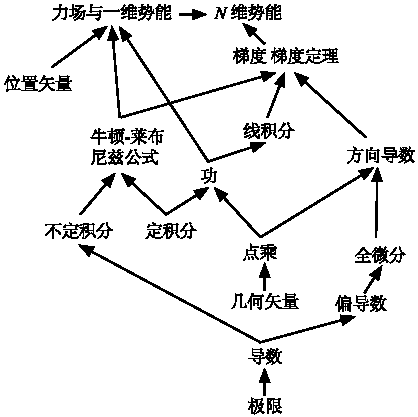
\includegraphics[width=10cm]{./figures/648204cc09583468.pdf}
\caption{由 “预备知识” 画出的知识树(目标文章为“力场、势能”)}\label{fig_about_1}
\end{figure}

完整的知识树见 \href{https://wuli.wiki/tree}{wuli.wiki/tree}, 可以选中任意节点为\textbf{目标节点},生成\textbf{子知识树}。 用计算机的术语,知识树是一个\textbf{有向无环图(DAG)},可以进行拓扑排序。 % \addTODO{两个链接}

一篇文章可包含一个或多个节点,文章中\textbf{每个 “预备知识” 列表就是一个节点的开始},如果 “预备知识” 中列出的内容都已经掌握,就可以开始学习该节点的内容,否则就先掌握 “预备知识” 中的内容。 若一篇文章中有多个节点,则每个节点都默认依赖前一个节点。

如果用 $A\to B$ 来表示节点 $A$ 是节点 $B$ 的预备知识, 或者称为 $B$ 的依赖, 把 $A$ 的所有依赖也叫做 $B$ 的依赖。 我们规定知识树不能出现类似这样的结构: $A \to B \to \dots \to C$ 且 $A \to C$, 因为这里的 $A \to C$ 是多余的。 而这样的结构是可以出现的: $A \to B_1 \to \dots \to C$ 且 $A \to B_2 \to \dots \to C$,我们把它称为棱形结构。 所以目录树种的棱形是不可避免的, 这可能导致整个目录树看起来结构并没有那么清晰。

依赖爆炸是知识树最可能出现的问题,也是下面一些概念努力想要解决的问题。

\subsubsection{自洽}
\textbf{自洽(self-contained)}。 一本教材的自洽性指目标读者在学习前是否还需要学习其他教材。 例如大部分本科物理教材对高中生都是不自洽的, 因为它们往往假设读者具有一定的微积分和线性代数基础。从微观来说,一个节点的自洽性体现在严格禁止出没有介绍过的、预备知识以外的术语或定理等。 自洽的具体要求是每个节点中的术语、定义和定理等必须来自本节点或预备知识。 对于后者,正文第一次出现时要给出具体且符合语境的链接,方便读者复习。

\subsubsection{多版本}
相对于百科或综述而言, 教材的内容编排是高度主观且取决于作者和目标读者的。 把同一个话题以不同深度, 严谨度和适用范围等划分成若干个等级的同名文章。 例如同一个数学或物理概念在高中生、大学生或研究生课程中有完全不同的表述方式。

小时百科中每篇文章的标题必须是全站唯一的, 若同一个话题有不同版本的文章, 我们使用稍微不同的标题或在它后面用括号加以区分。 例如 “角动量(科普)”, “角动量、角动量定理、角动量守恒(单个质点)”, “角动量定理、角动量守恒”, “轨道角动量(量子力学)”, “自旋角动量” 都分布在不同的部分和章节。

又例如 “对称矩阵的本征问题” 和 “厄米矩阵的本征问题” 内容几乎相同,只是后者把对实数的称矩阵推广到了复数的厄米矩阵,虽然后者完全包含前者,但为了照顾特定读者仍然划分两个版本。 这个例子也体现了下文的特殊到一般思想。


一个经常遇到的问题是, 有时候一篇文章的范围很难明确界定。 例如 “球谐函数” 页面, 如果它本来是作为某个其他页面的预备知识而创作的一个连贯自洽的小教程, 它不会像维基百科的\href{https://en.wikipedia.org/wiki/Spherical_harmonics}{球谐函数条目}那样包含几乎所有性质以及和其他众多特殊函数的关系, 而只是包含一些在某个场景下比较重要的性质(例如解氢原子的定态波函数所需要的那些)以及特定的讲解方式和举例。 但是随着其他需要使用球谐函数作为预备知识的页面的出现, 原作者或其他人可能会倾向于不断往同一个页面补充并引用新的性质, 并调整讲解顺序, 最后导致其越来越接近维基百科——但这样它就变得不那么连贯或适合初学/自学了。 可见百科和教材存在不可调和的矛盾。 对于一个话题, 我们不可能写出一个既像教材又像百科的 “部分” 并让所有人都满意。

我们解决该问题的方法就是多版本,为量子力学而写的球谐函数文章确定好范围和讲解顺序后就不再改变,若其他学科需要另一个范围或讲解方式就新创建一个版本或者以已有版本为预备知识并补充新的内容。要强调的是,我们\textbf{无需避免相似的内容在不同版本的文章重复出现}, 如果协议兼容,我们可以把一个版本中的内容直接复制到另一个版本并进行修改。

所有关于球谐函数的性质总结归类后,放入类似维基百科的综述版本。综述版本只起到总结归纳作用,方便已经学过的人查阅检索, 不包含太多具体的细节和推导,不必照顾初学者。 综述版本省略的细节可以链接到其他他版本的具体位置。

最后,不同的球谐函数页面就会分别被命名为诸如 “球谐函数(综述)”, “球谐函数简介(量子力学)”, “球谐函数表”, “球谐函数与XXX”, “球谐函数的XX性质” 等等。

\subsubsection{封装和分离}
这里的封装借用了面对对象编程的概念。在面对对象编程中,一个对象的使用方法和它的内部实现是严格分离的。使用者只需要了解对象使用方法而不需要了解对象内部的运作机制。在小时百科中,该思想最典型的应用就在介绍一个定理时,把 “是什么”、“有什么用”、 “如何使用” 和 “如何证明” 划分为不同的节点。 这样只想了解前者的读者就可以跳过后者。

例如傅里叶变换的使用方法和严格证明所需要的预备知识大不相同,前者通常在普通微积分教材中出现,而后者需要学习实变函数、泛函分析等数学专业才会涉及到的高级内容。如果不把它们分开成不同的节点,那么想要学习前者的人将会面临大量多余的预备知识。

一些教材会抱着和读者一起探索的思想,先不直接给出结论,而是在推导过程中一步步得到想要的结论。而我们认为除了有这样的讲解之外,还应该把其中的关键结论提取出来放在推到之前作为单独的节点,给那些只想使用而不想深入了解原理的读者提供方便。

\subsubsection{特殊到一般}
例如在线性代数中,我们倾向于先讲解二维和三维的几何向量及其运算如加法、数乘、点乘等运算, 然后才引入线性组合、线性变换、实数矩阵、复数矩阵、线性空间等概念。这是符合大部分初学者学习规律的方式。 适用范围更广的节点应该以更形象易学、适用范围更窄的节点作为预备知识。

反之,线性代数无论从矩阵的行变换和行列式开始,还是首先给出线性空间的完整定义,都是违反教学规律的。

\subsubsection{目录}
我们\textbf{强调知识树而弱化目录}。

在小时百科的\href{https://wuli.wiki/online}{目录}中, 我们并不是按照话题来分类所有, 而是创建许多\textbf{部分}。 有的部分可以是一个非常完整和连续的传统教材, 适合按顺序从头读到尾(当然你也可以根据依赖关系自己决定读哪些)。 而另一些部分则没那么系统, 只是把某个话题下一些相对独立的小教程、博文、讲义、笔记等放到一起(但仍然需要给出具体的依赖关系)。 至于维基百科那样的综述性条目, 我们同样可以根据话题创建\textbf{专门的部分}来收纳它们, 这些综述的正文中又可以进一步链接到其他部分中的页面(例如详细的证明推导)。 小时百科的每个部分(甚至它的每章)都应该有介绍页面来描述它的内容和结构。每部分尽量按照拓扑排序,即每个节点的预备知识必须排在它的前面。

% === 这段应该放到 “创作指导” 中, 这篇文章是给读者看的 ====
% 每个页面应该有对应的审核员(通常是该页面的第一作者)来负责, 其他人想修改或添加内容需要经过他同意, 如果审核者认为要添加的内容超出了本文的范围, 则应该另外创建一个页面。 不应该像百科(综述)一样, 众多不同的人把众多不同的内容塞进同一个页面。

% ========= 回收的内容 ===========
% 如果我们只有一本公认优秀的传统教材,它包含了丰富的导入,动机,定义,定理,讲解,例题,习题。 而且它有一个很明确的目标人群,这些内容的深度和讲解思路,严谨性,都是为这个人群定制的。

% 那么,如何在一字不变的情况下把它做成灵活的模块化结构呢?

% 这样,我们可以把任意一本教材的内容切割并赋予一个树状结构。 就相当于给这本书生成一个知识地图。 书的内容一字不变,但是读者通过地图很容易看出来全书的结构。 一个极端的例子是,整本书都是严格线性的,任意第 $i+1$ 个节点都需要第 $i$ 个节点作为预备知识。 那么所谓的树状图就只有一个分支,这就要求所有读者把整本书从头看到尾或者看到中间的某个节点。 但几乎没有一本教材是这样严格的结构,它通常有许多不同的话题, 例如教材第一节是理论基础 A, 而第二节和第三节分别是话题 B 和话题 C, B 和 C 之间并没有什么联系, 可能一些读者只需要 B 另一些只需要 C。 在没有树状图时,读者并不知道看完 A 就可以直接看 C, 给出树状图以后读者就知道 B 是可以省略的。
